% Options for packages loaded elsewhere
\PassOptionsToPackage{unicode}{hyperref}
\PassOptionsToPackage{hyphens}{url}
%
\documentclass[
  10pt,
  ignorenonframetext,
  a4paper,handout]{beamer}
\usepackage{pgfpages}
\setbeamertemplate{caption}[numbered]
\setbeamertemplate{caption label separator}{: }
\setbeamercolor{caption name}{fg=normal text.fg}
\beamertemplatenavigationsymbolsempty
% Prevent slide breaks in the middle of a paragraph
\widowpenalties 1 10000
\raggedbottom
\setbeamertemplate{part page}{
  \centering
  \begin{beamercolorbox}[sep=16pt,center]{part title}
    \usebeamerfont{part title}\insertpart\par
  \end{beamercolorbox}
}
\setbeamertemplate{section page}{
  \centering
  \begin{beamercolorbox}[sep=12pt,center]{part title}
    \usebeamerfont{section title}\insertsection\par
  \end{beamercolorbox}
}
\setbeamertemplate{subsection page}{
  \centering
  \begin{beamercolorbox}[sep=8pt,center]{part title}
    \usebeamerfont{subsection title}\insertsubsection\par
  \end{beamercolorbox}
}
\AtBeginPart{
  \frame{\partpage}
}
\AtBeginSection{
  \ifbibliography
  \else
    \frame{\sectionpage}
  \fi
}
\AtBeginSubsection{
  \frame{\subsectionpage}
}
\usepackage{lmodern}
\usepackage{amssymb,amsmath}
\usepackage{ifxetex,ifluatex}
\ifnum 0\ifxetex 1\fi\ifluatex 1\fi=0 % if pdftex
  \usepackage[T1]{fontenc}
  \usepackage[utf8]{inputenc}
  \usepackage{textcomp} % provide euro and other symbols
\else % if luatex or xetex
  \usepackage{unicode-math}
  \defaultfontfeatures{Scale=MatchLowercase}
  \defaultfontfeatures[\rmfamily]{Ligatures=TeX,Scale=1}
\fi
% Use upquote if available, for straight quotes in verbatim environments
\IfFileExists{upquote.sty}{\usepackage{upquote}}{}
\IfFileExists{microtype.sty}{% use microtype if available
  \usepackage[]{microtype}
  \UseMicrotypeSet[protrusion]{basicmath} % disable protrusion for tt fonts
}{}
\makeatletter
\@ifundefined{KOMAClassName}{% if non-KOMA class
  \IfFileExists{parskip.sty}{%
    \usepackage{parskip}
  }{% else
    \setlength{\parindent}{0pt}
    \setlength{\parskip}{6pt plus 2pt minus 1pt}}
}{% if KOMA class
  \KOMAoptions{parskip=half}}
\makeatother
\usepackage{xcolor}
\IfFileExists{xurl.sty}{\usepackage{xurl}}{} % add URL line breaks if available
\IfFileExists{bookmark.sty}{\usepackage{bookmark}}{\usepackage{hyperref}}
\hypersetup{
  pdftitle={Infodemiology\ldots\ldots.},
  pdfauthor={Andrzej Jarynowski, Vitaly Belik},
  hidelinks,
  pdfcreator={LaTeX via pandoc}}
\urlstyle{same} % disable monospaced font for URLs
\newif\ifbibliography
\setlength{\emergencystretch}{3em} % prevent overfull lines
\providecommand{\tightlist}{%
  \setlength{\itemsep}{0pt}\setlength{\parskip}{0pt}}
\setcounter{secnumdepth}{-\maxdimen} % remove section numbering

\setbeamertemplate{footline}[page number]
\setbeamertemplate{navigation symbols}{}
\usecolortheme{lily}%seahorse}
%\setbeamertemplate{footline}[frame number]{}
\usepackage{xcolor}
\usepackage{amssymb}
%\titlegraphic{\includegraphics[width=0.3\paperwidth]{\string~/Dropbox/teaching/clemson-academic.png}}
\definecolor{beamer}{RGB}{51,51,178}
\ifluatex
  \usepackage{selnolig}  % disable illegal ligatures
\fi

\title{Infodemiology\ldots\ldots.}
\author{Andrzej Jarynowski, Vitaly Belik}
\date{26.10.2020}
\institute{Institute of Veterinary Epidemiology and Biostatistics, Freie
Universität Berlin, Germany}

\begin{document}
\frame{\titlepage}

\begin{frame}{Outline}
\protect\hypertarget{outline}{}
\Large
\pause

\begin{enumerate}
[1)]
\item
  Introduction to infodemiology (the traditional and social-content
  media on the Internet in pandemic)
\item
  Examples then infodemiology supporting and supplementing traditional
  public health repertoire
\item
  Examples then infosurvelliance could supress traditional medical
  reasearch (clinical trials and registries)
\item
  Roadmap for analysis of German Internet
\end{enumerate}

\large

\pause
\end{frame}

\begin{frame}{Infodemic}
\protect\hypertarget{infodemic}{}
\begin{itemize}
\tightlist
\item
  traditional vs social-content media
\item
  a concept in the social medicine area: ``lay-referral framing system''
  where opinions and beliefs of the general public are something
  different from medical knowledge.
\item
  information is widely treated as a trigger of consequences impacting
  daily-life security
\item
  participatory epidemiology
\end{itemize}
\end{frame}

\begin{frame}{History of Infodemiology and infosurvelliance}
\protect\hypertarget{history-of-infodemiology-and-infosurvelliance}{}
\begin{itemize}
\item
  Google Flu Trends (2010) - syndromic infosurvelliance using ILI
  keywords.
\item
  Infosurvelliance in prediction/forecasting COVID-19 infection dynamics
  worked far below expectation in Europe for publicly availabe dataset
  (i.e.~Lampos, Vasileios, et al.~``Tracking COVID-19 using online
  search.'' NPJ digital medicine 4.1 (2021): 1-11.), but seems to work
  with much more precised dataset in China (i.e.~Guo, Shuhui, et
  al.~``Improving Google flu trends for COVID-19 estimates using Weibo
  posts.'' Data Science and Management 3 (2021): 13-21.)
\item
  High expectation, little predictive power (low digitalization rates
  and lack of availability of individual records in Western societies?)
\end{itemize}
\end{frame}

\begin{frame}{Infodemiology as supporting tool for public health}
\protect\hypertarget{infodemiology-as-supporting-tool-for-public-health}{}
\begin{itemize}
\item
  Meassuring the social interest in/around SARS-CoV-2 and COVID-19 in
  the Internet media during the epidemic
\item
  Quantifing dynamics of interest (demand and supply of content) and
  discourse patterns.
\item
  Internet as a digital footprint of social activities (secondary
  document analysis)
\item
  Media Analysis of the social proceses. SEO-marketing solutions as
  SentiOne (used by Infodemic menagment by WHO)
\item
  Serves as a complement to longitudinal surveys monitoring public
  perception (and other socio-economic methods) in REAL TIME
\end{itemize}
\end{frame}

\begin{frame}{WHO Infodemiological intelligence}
\protect\hypertarget{who-infodemiological-intelligence}{}
Part of Hub for Pandemic and Epidemic Intelligence in Berlin

\begin{center}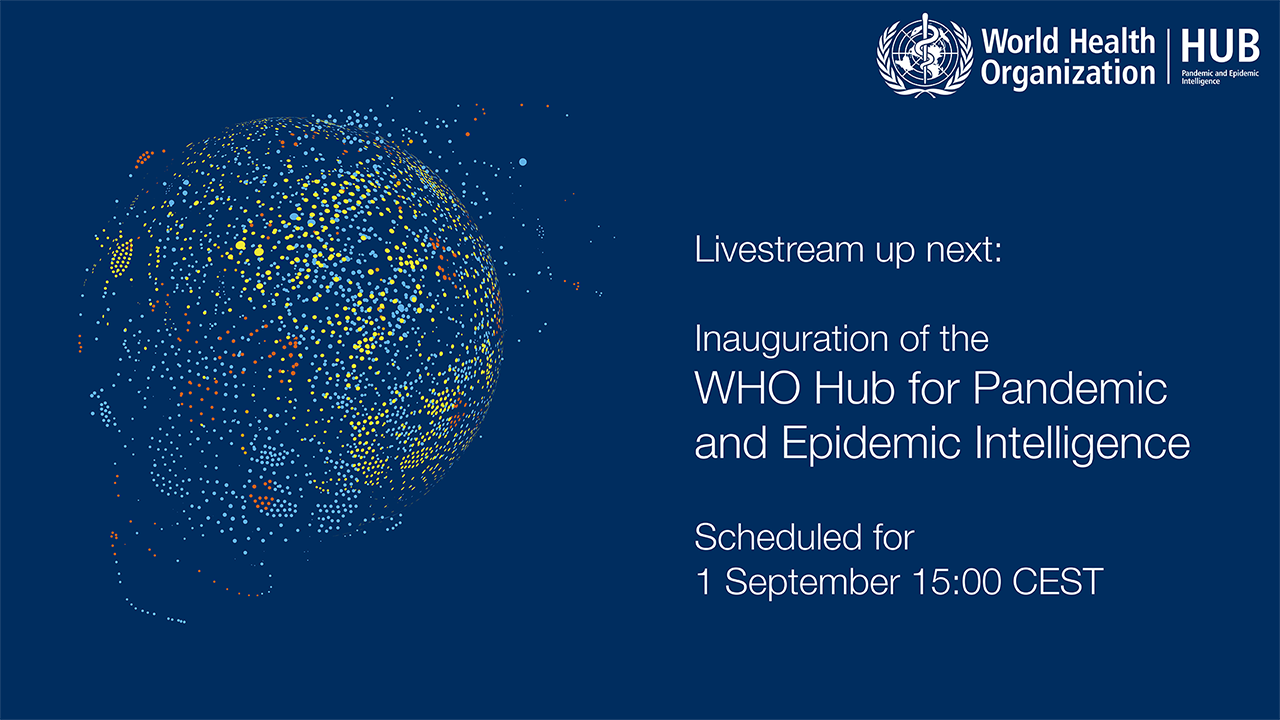
\includegraphics[width=0.7\linewidth]{who_20210901_101_en} \end{center}

\url{https://www.who.int/news/item/01-09-2021-who-germany-open-hub-for-pandemic-and-epidemic-intelligence-in-berlin}
\end{frame}

\begin{frame}{Methodologies and goels}
\protect\hypertarget{methodologies-and-goels}{}
\begin{center}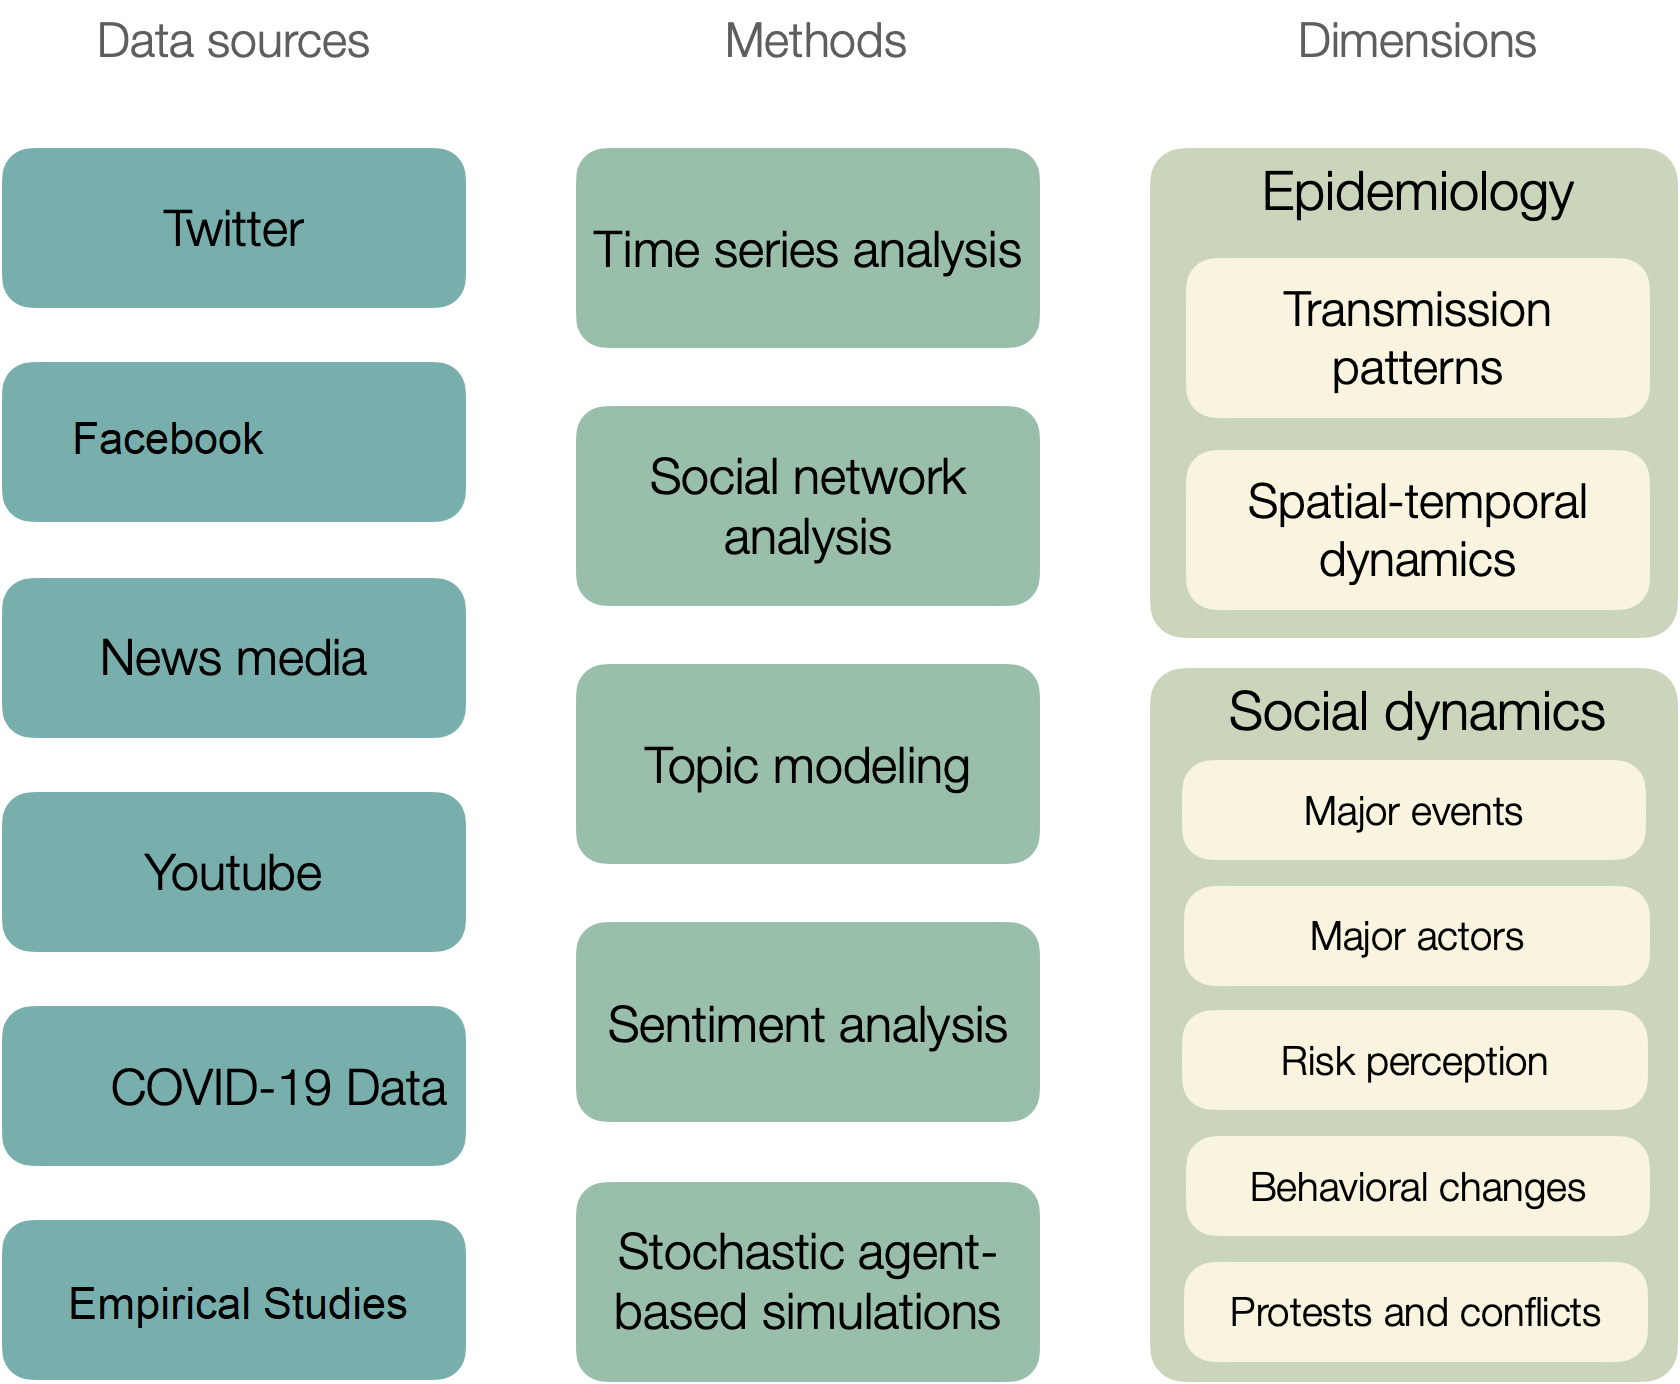
\includegraphics[width=0.7\linewidth]{scheme} \end{center}

Scheme of the proposed infodemiological project, We aim to infer the
interplay between social dynamics as revealed via Internet media and
epidemiology of COVID-19 (only major data sources are shown) deploying
the methods presented.
\end{frame}

\begin{frame}{Think globally, act locally}
\protect\hypertarget{think-globally-act-locally}{}
\begin{itemize}
\tightlist
\item
  What? (content (key vocabulary, topics and sentiment) as on risk
  communication, fake news etc.)
\item
  Who? (categories of senders of information, Who are main actors and
  communities in discourse)
\item
  When? (timeline, how does perception of disease evolve?),
\item
  Where? (geography, cross-regional comparison)
\item
  How? (providing new information or blocking existing channels, Which
  factors affect risk perception and adherence to NPI?)
\end{itemize}
\end{frame}

\begin{frame}{Outline}
\protect\hypertarget{outline-1}{}
\Large
\pause

\begin{enumerate}
[1)]
\tightlist
\item
  Introduction to infodemiology (the traditional and social-content
  media on the Internet in pandemic)
\end{enumerate}

\textbf{2) Examples then infodemiology supporting and supplementing
traditional public health repertoire}

\begin{enumerate}
[1)]
\setcounter{enumi}{2}
\item
  Examples then infosurvelliance could supress traditional medical
  reasearch (clinical trials and registries)
\item
  Roadmap for analysis of German Internet
\end{enumerate}

\large

\pause
\end{frame}

\begin{frame}{Topic Modelling of News in Poland}
\protect\hypertarget{topic-modelling-of-news-in-poland}{}
Social aspects are dominating!

\begin{center}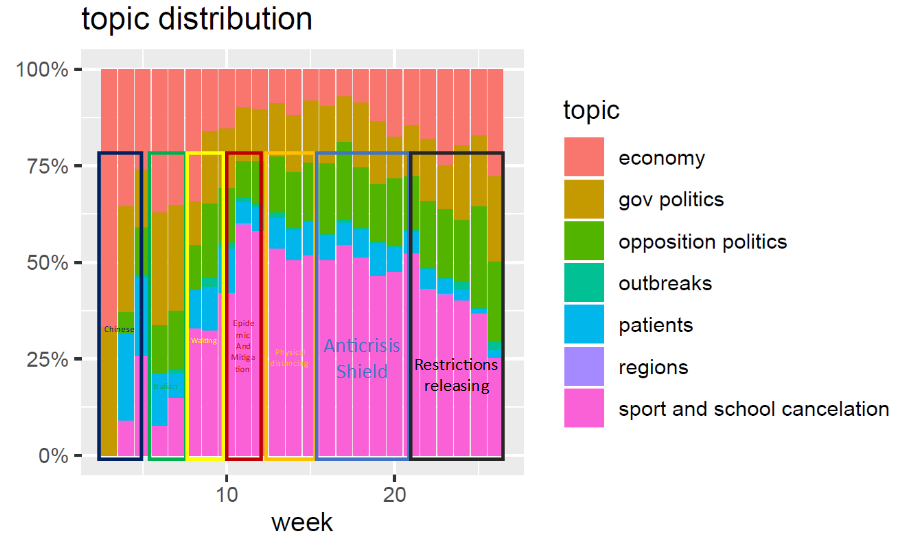
\includegraphics[width=1\linewidth]{top} \end{center}

Weekly dynamics of media perception in Poland. Main Topics in over 50
thousand news articles (without garbage codes).
\end{frame}

\begin{frame}{Interest in ``Coronavirus'' in Poland (multiple media
source)}
\protect\hypertarget{interest-in-coronavirus-in-poland-multiple-media-source}{}
\begin{center}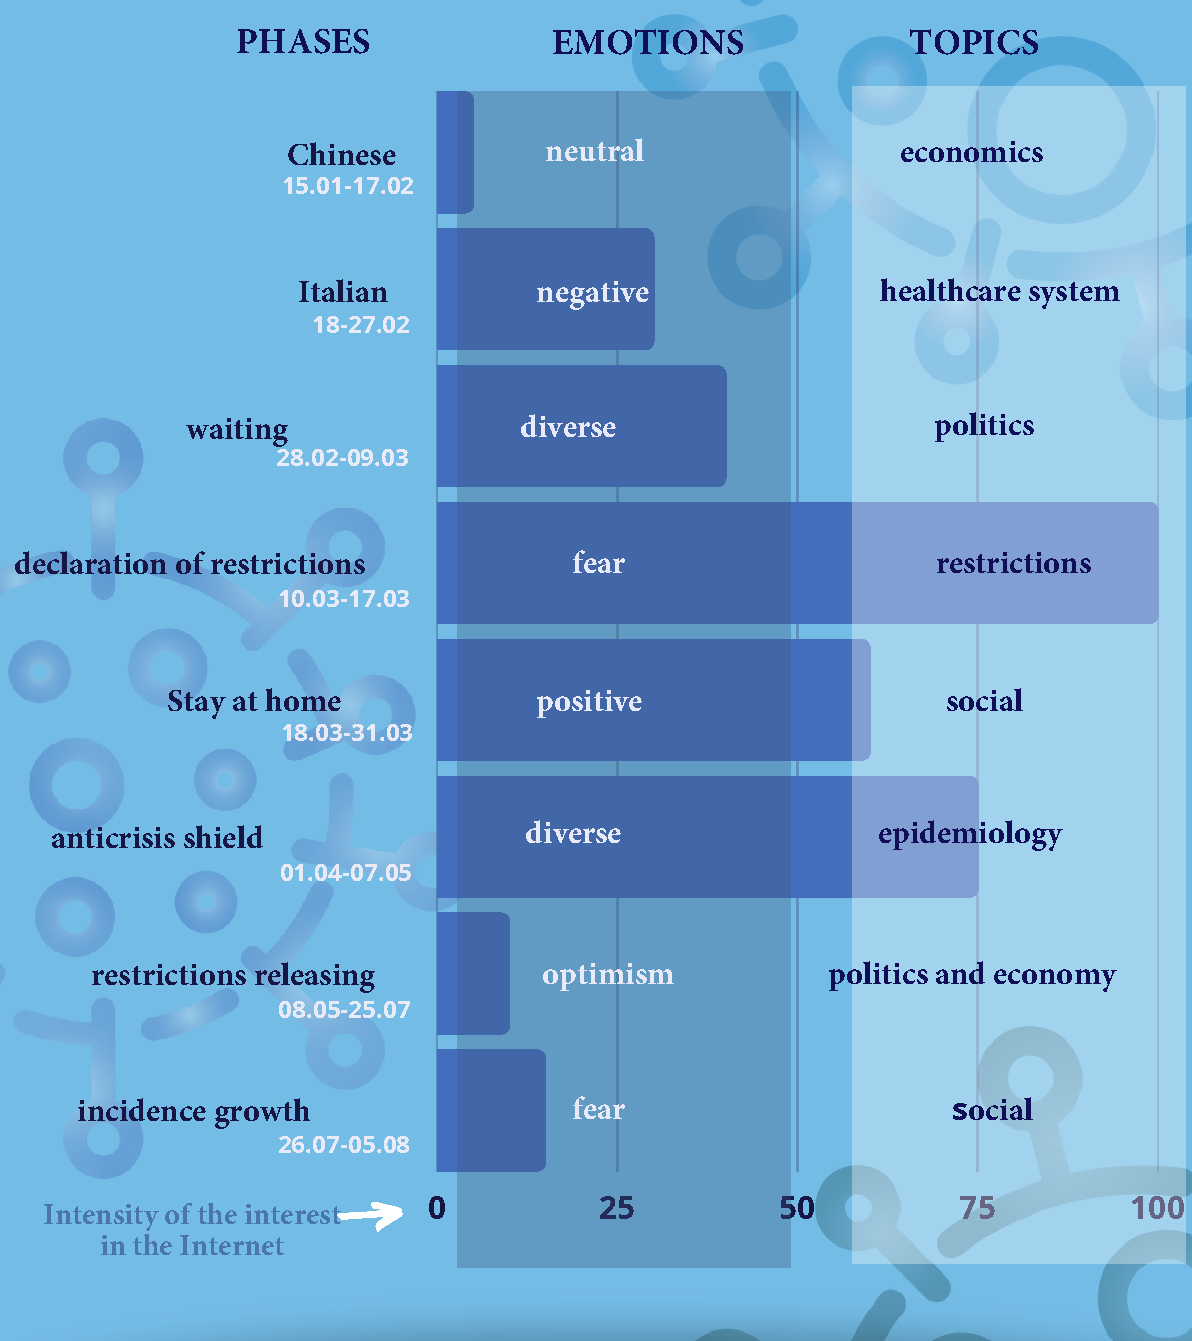
\includegraphics[width=0.5\linewidth]{phases} \end{center}

Jarynowski, Andrzej, Monika Wójta-Kempa, and Vitaly Belik. ``Trends in
interest of COVID-19 on Polish Internet.'' Epidemiol Rev 74 (2020):
258-275.
\end{frame}

\begin{frame}{Polarization in Polish Twitter}
\protect\hypertarget{polarization-in-polish-twitter}{}
The (de-)polarization (revealed by modularity and sentiment analysis)

\begin{center}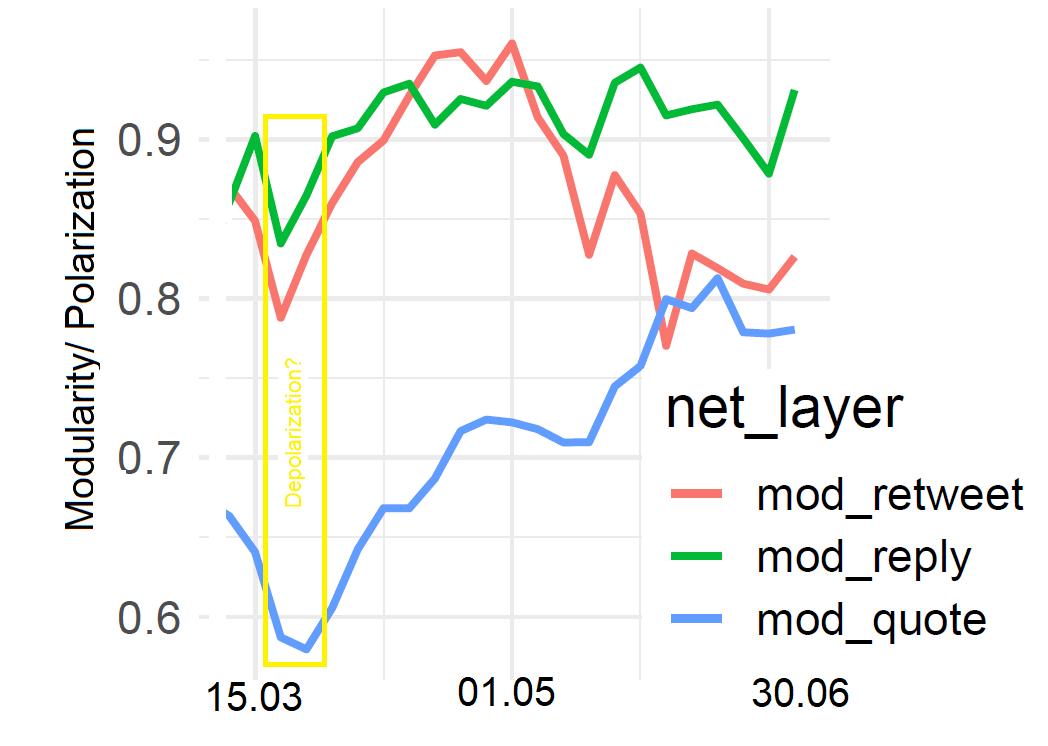
\includegraphics[width=0.5\linewidth]{polaryzacja} \end{center}

Modularity of the full networks (over 30 thousands accounts) and their
weekly dynamics for different type of communication relations
(retweeting, reply, quotation).

Jarynowski, Andrzej, et al.~``Social Cohesion During the Stay-at-Home
Phase of the First Wave of the COVID-19 Pandemic on Polish-Speaking
Twitter.'' LNCS in press (2021).
\end{frame}

\begin{frame}{Outline}
\protect\hypertarget{outline-2}{}
\Large
\pause

\begin{enumerate}
[1)]
\item
  Introduction to infodemiology (the traditional and social-content
  media on the Internet in pandemic)
\item
  Examples then infodemiology supporting and supplementing traditional
  public health repertoire
\end{enumerate}

\textbf{3) Examples then infosurvelliance could supress traditional
medical reasearch (clinical trials and registries) }

\begin{enumerate}
[1)]
\setcounter{enumi}{3}
\tightlist
\item
  Roadmap for analysis of German Internet
\end{enumerate}

\large

\pause
\end{frame}

\begin{frame}{Sputnik V}
\protect\hypertarget{sputnik-v}{}
\begin{center}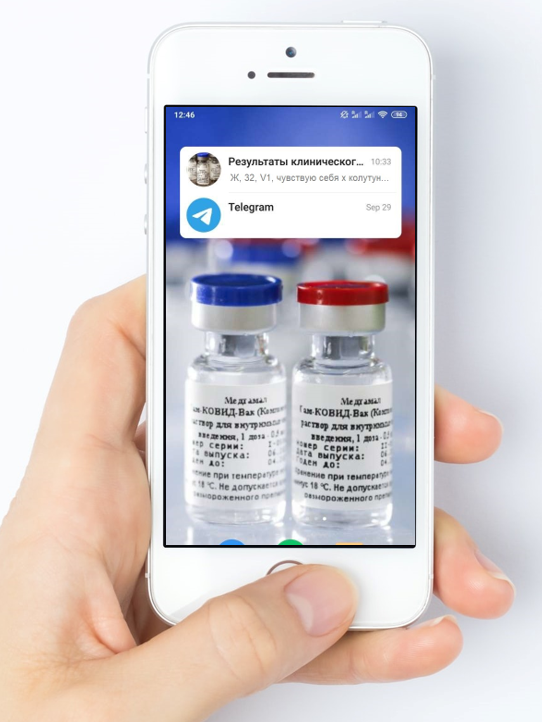
\includegraphics[width=0.7\linewidth]{Picture4to3} \end{center}
\end{frame}

\begin{frame}{Outline}
\protect\hypertarget{outline-3}{}
\Large
\pause

\begin{enumerate}
[1)]
\item
  Introduction to infodemiology (the traditional and social-content
  media on the Internet in pandemic)
\item
  Examples then infodemiology supporting and supplementing traditional
  public health repertoire
\item
  Examples then infosurvelliance could supress traditional medical
  reasearch (clinical trials and registries)
\end{enumerate}

\textbf{4) Roadmap for analysis of German Internet }

\large

\pause
\end{frame}

\begin{frame}{Protest in Berlin (Twitter)}
\protect\hypertarget{protest-in-berlin-twitter}{}
We have collected tweets in German language with hashtags B0108 (92,474)
and B2908 (345,992) for both main demonstrations on August 1st and
August 29th, 2020 in Berlin.

For Twitter data we can deploy the temporal network analysis of users
(here retweets), and simple NLP.

Jarynowski, Andrzej, Alexander Semenov, and Vitaly Belik. ``Protest
perspective against COVID-19 risk mitigation strategies on the German
Internet.'' International Conference on Computational Data and Social
Networks. Springer, Cham, 2020.
\end{frame}

\begin{frame}{Protest in Berlin (01.08.2020) on Twitter}
\protect\hypertarget{protest-in-berlin-01.08.2020-on-twitter}{}
\begin{center}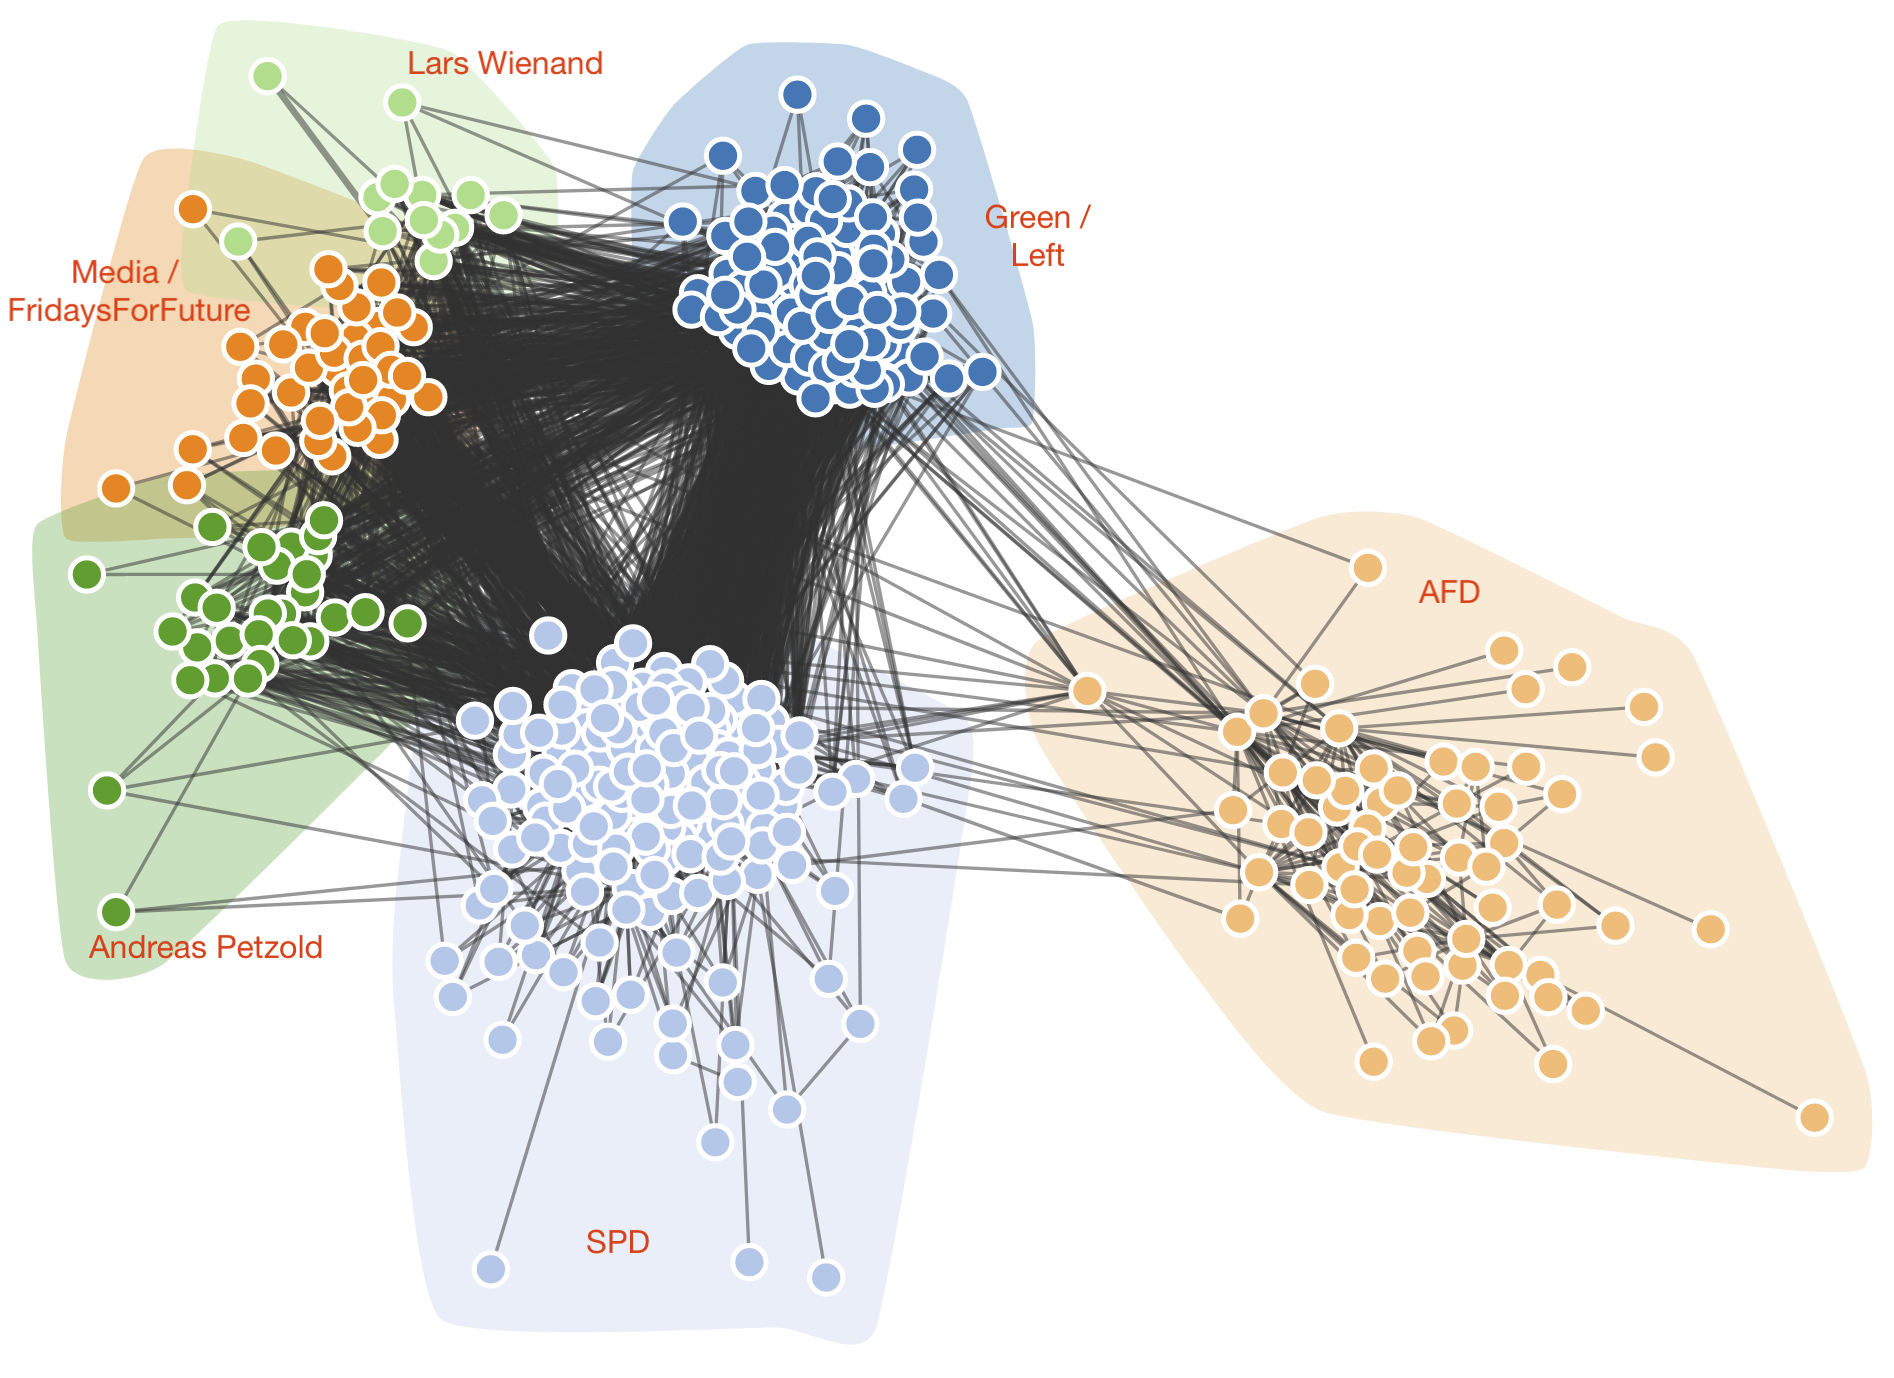
\includegraphics[width=0.85\linewidth]{b0108_comminities} \end{center}

We observe such a mosaic pattern in German protests when representatives
of AfD party as well as the SPD and the Green parties were connected on
the retweet network during 01.08.2020 Berlin protests with hashtag b0108
\end{frame}

\begin{frame}{Protest in Berlin (29.08.2020) on Twitter}
\protect\hypertarget{protest-in-berlin-29.08.2020-on-twitter}{}
\begin{center}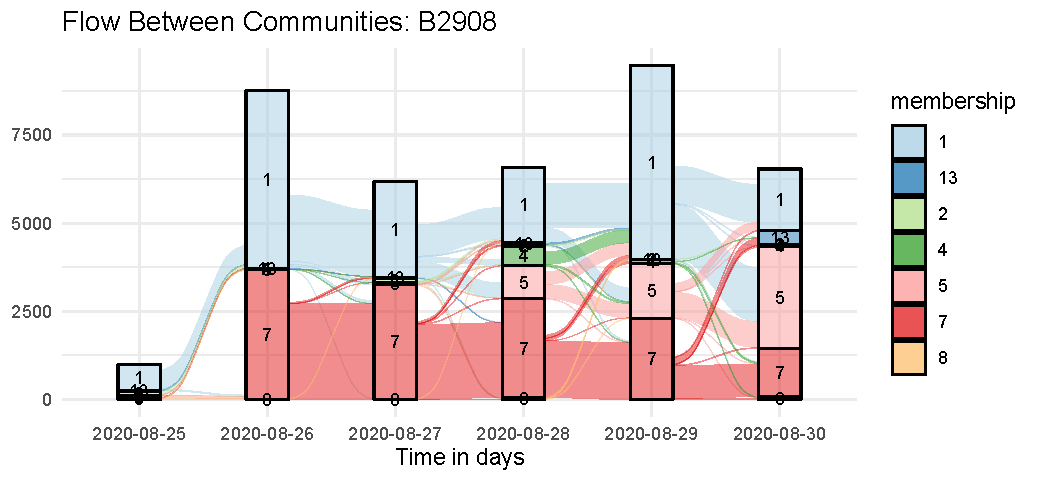
\includegraphics[width=0.95\linewidth]{b29_flow_} \end{center}

Flow of users between communities with the biggest communities on the
retweet network. Codes for the main identified communities: 1 -- SPD and
mainstream (anti-protest); 5 -- Antifa (anti-protest); 7-- AfD
(pro-protest); 4 -- community of left-wing liberals (anti-protest); 13
-- liberal and more acceptable to protests
\end{frame}

\begin{frame}{Vaccine context on German Twitter}
\protect\hypertarget{vaccine-context-on-german-twitter}{}
Net of hashtags and actors
\end{frame}

\begin{frame}{Conclusions}
\protect\hypertarget{conclusions}{}
\begin{itemize}
\item
  The COVID-19 epidemic in the Internet is primarily of a social, not
  medical, dimension;
\item
  Role Social media in driving social processes doesn't need to be
  always negative;
\item
  Infodemiology \textbf{is very usefull} in understanding social
  dynamics during pandemic a supplementary role to standard tools as
  surveys;
\item
  Infosurvelliance \textbf{could be usefull} for public health decision
  makers in some specific areas too.
\end{itemize}
\end{frame}

\end{document}
